\chapter{Results}

This chapter presents the experimental results from the implementation. The
experiments are not intended to propose a secure cryptosystem or to recommend
secure parameters, because the classical constructions discussed in this thesis
are already known to be vulnerable. The goal is to check that the
implementation works correctly, to compare the running time of the implemented
variants, and to illustrate how selected parameters influence the generated
knapsack instances.

\section{Experimental Setup}

The experiments were run with the C implementation described in the previous
chapter. The benchmark mode measures key generation, encryption, and decryption
separately and prints the results in CSV format. The experiment scripts ran the
compiled program with selected parameters and stored its CSV output in
\texttt{experiments/results}. The plots used in this chapter were then
generated from these CSV files by the plotting script. The same scripts were
also run on a macOS machine as a sanity check, but only the Linux measurements
are reported here.

For the cryptographic benchmarks, the tested block sizes were
\[
    n \in \{128,256,512,1024,2048,4096\}.
\]
The program reports density from the bit length of the largest public weight.
This is close to the density definition used in Chapter~2, because the bit
length tells how many binary digits are needed to represent the largest weight.
This is the same size information that the base-two logarithm measures. The
value is used only for comparing the generated instances in these experiments.
When the largest public weight needs more bits and the block size \(n\) stays
the same, the reported density becomes lower.

Each configuration was tested with three deterministic seeds. For each seed,
the benchmark used five measured repetitions after three warm-up repetitions.
The compared schemes were \texttt{mh-classic}, \texttt{mh-permuted}, and
\texttt{mh-iterated}. The final measurements were run on a desktop computer
running Linux with an Intel Core i9-10850K CPU. The program was compiled with
GCC 16.1.1 using the C11 standard and linked with GMP 6.3.0. 

A separate sweep was also run for the iterated variant. In this experiment, the
number of total modular transformation layers was changed to
\[
    L \in \{2,3,4,5\}.
\]
The layer count was set with the \texttt{--layers} option, while the same
block sizes and deterministic seeds were used. This experiment was included
to show how additional modular layers affect runtime and the density of the
public knapsack.

The attack experiments used only the public knapsack instance of the classical
Merkle--Hellman scheme. The implemented solvers are brute-force search and
meet-in-the-middle search. They are included only as simple subset-sum solvers.
They are not implementations of Shamir's polynomial-time attack or of
lattice-based low-density attacks.

\section{Correctness of the Implementation}

Correctness was checked by encrypting an input message and then decrypting the
resulting ciphertext. In each benchmark run, the decrypted bit sequence was
compared with the original input before the timing result was accepted. The same
check was also used in demo mode for raw bit strings and for plaintext messages
that are converted into bit blocks before encryption.

The automated test script builds the address-sanitized version of the program
and runs the three implemented variants on small examples. It also checks that
benchmark mode produces CSV output, that the simple subset-sum solvers recover
small generated messages, and that selected invalid inputs are rejected. These
tests are not a formal verification, but they check the main workflows used in
the experiments.

\section{Runtime of Implemented Variants}

Figure~\ref{fig:crypto-total-ms} compares the total running time of the three
implemented variants. The total time is the sum of key generation, encryption,
and decryption for one fixed-size block. The measured times are small, so the
exact ordering for the smallest block sizes should not be overinterpreted.
However, the growth with increasing \(n\) is visible.

For example, the average total time of the classical variant increased from
about \(0.016\) ms for \(n=128\) to about \(11.057\) ms for \(n=4096\). The
permuted variant had similar behaviour, because the permutation changes the
order of the weights but does not change the main arithmetic operations. The
default iterated variant became slower for larger block sizes. For \(n=4096\),
its average total time was about \(30.929\) ms. This is expected, because it
applies an additional modular transformation layer.

\begin{figure}[htbp]
    \centering
    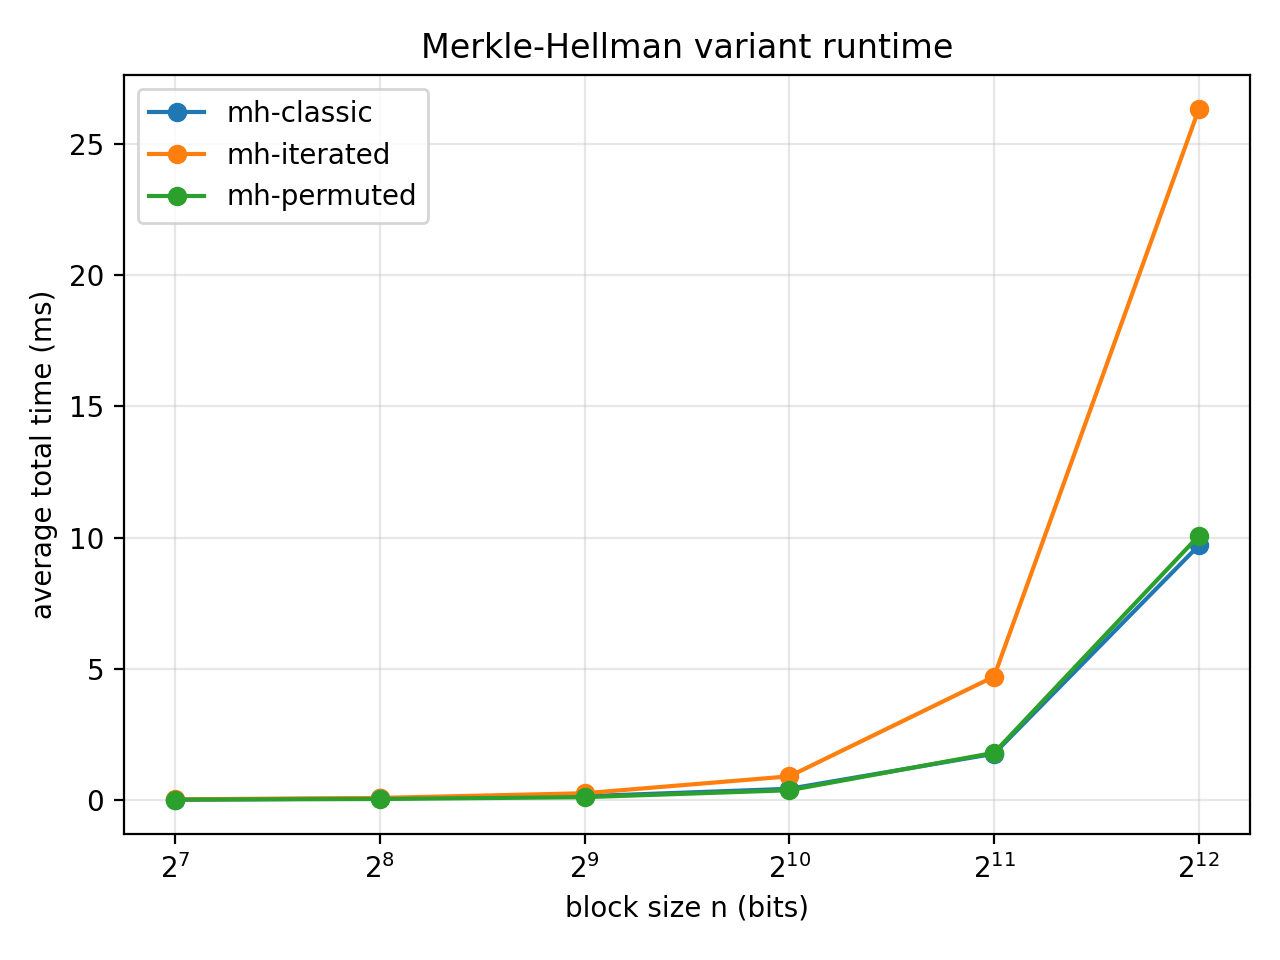
\includegraphics[width=0.9\textwidth]{../code/experiments/plots/crypto_total_ms.png}
    \caption{Average total runtime of the implemented Merkle--Hellman variants.}
    \label{fig:crypto-total-ms}
\end{figure}

Figure~\ref{fig:crypto-components-classic} shows the operation breakdown for
the classical variant. In this implementation, key generation is the largest
part of the measured runtime. At \(n=4096\), the average key-generation time
was about \(10.895\) ms, while encryption took about \(0.089\) ms and
decryption about \(0.072\) ms. This difference is expected, because key
generation allocates and initializes the key material and constructs the
trapdoor. It generates the superincreasing private sequence, chooses a modulus
larger than the private sum, samples a multiplier \(r\) from the range \(2 \le
r < m\) until \(\gcd(r,m)=1\), computes the modular inverse of \(r\), and
builds all public weights. This cost could be changed by using a different
method for choosing parameters. For example, using a prime modulus would make
every non-zero multiplier invertible and could reduce the rejection step when
choosing \(r\). However, this would require choosing the modulus in a special
way and would change the distribution of generated keys, so it was not
evaluated in these experiments. Encryption and decryption are much quicker in
this benchmark. Encryption only adds the public weights corresponding to
message bits equal to \(1\). Decryption first uses the inverse of the
multiplier to transform the ciphertext back to a private subset sum, and then
solves this superincreasing subset-sum instance by the greedy algorithm. The
efficiency of these operations was one of the reasons why the Merkle--Hellman
construction was originally attractive.

\begin{figure}[htbp]
    \centering
    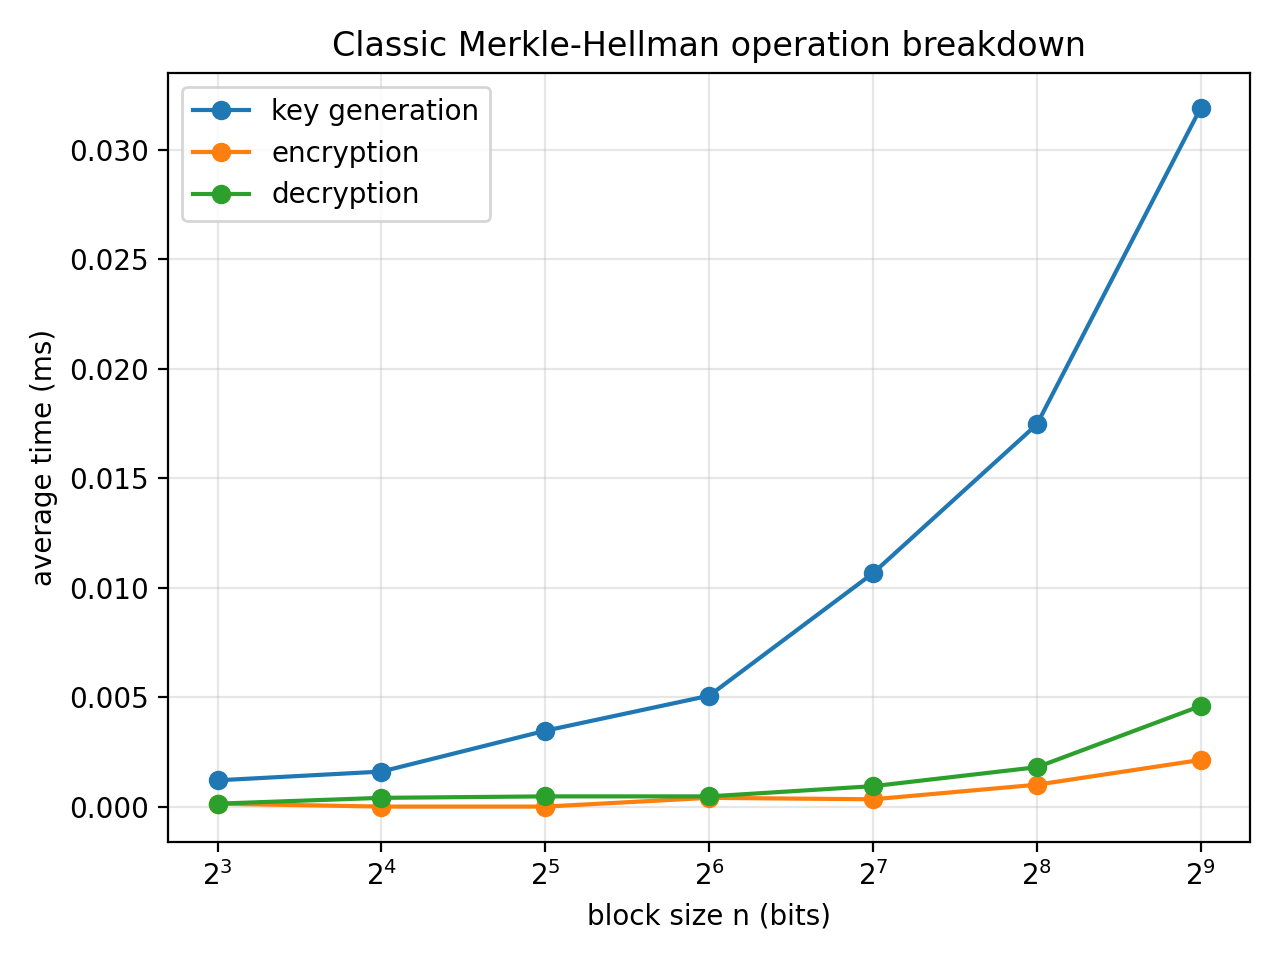
\includegraphics[width=0.9\textwidth]{../code/experiments/plots/crypto_components_classic.png}
    \caption{Runtime breakdown of the classical Merkle--Hellman implementation.}
    \label{fig:crypto-components-classic}
\end{figure}

\section{Effect of Additional Iterated Layers}

The iterated variant was also tested with a larger number of modular
transformation layers. This experiment is useful because historical iterated
knapsack constructions tried to hide the original superincreasing structure by
repeating the modular transformation. As discussed in the previous chapter,
this did not repair the security problem. In the implementation, additional
layers mainly increase the amount of modular arithmetic during key generation
and decryption.

Figure~\ref{fig:crypto-total-with-iterated-layers} compares the default
variants with iterated variants using more layers. The runtime increases as the
number of layers grows. For \(n=4096\), the average total time of the iterated
variant increased from about \(30.634\) ms with two layers to about \(88.693\)
ms with five layers. The increase is moderate for these experimental
parameters, but it shows the extra cost of applying more modular transformation
layers.

\begin{figure}[htbp]
    \centering
    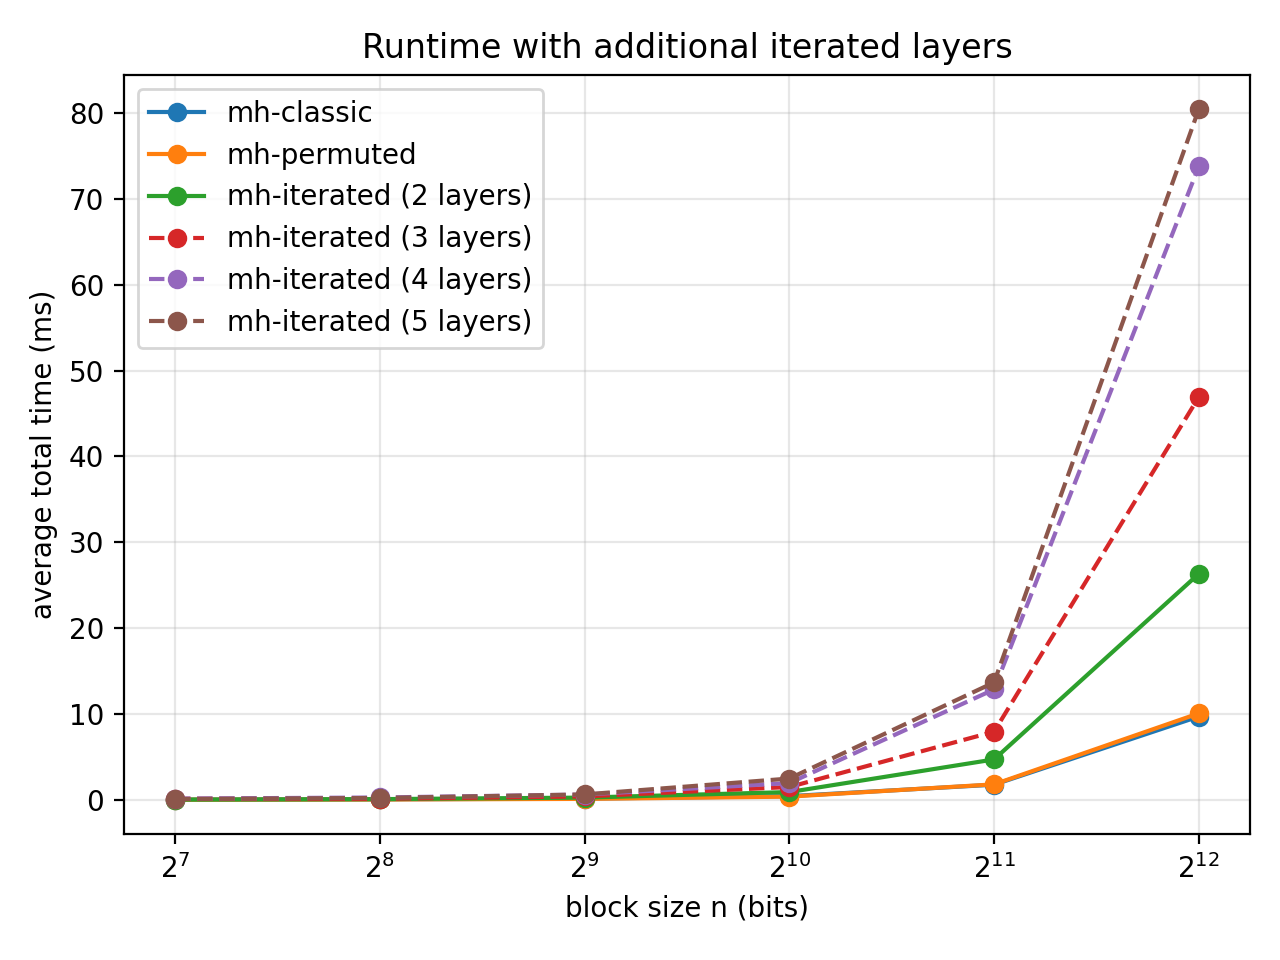
\includegraphics[width=0.9\textwidth]{../code/experiments/plots/crypto_total_with_iterated_layers.png}
    \caption{Runtime comparison including iterated variants with additional layers.}
    \label{fig:crypto-total-with-iterated-layers}
\end{figure}

Figure~\ref{fig:iterated-layers-density} shows the density of the iterated
variant for different layer counts. Adding more layers decreases the
measured density, because each additional modular transformation tends to
increase the bit length of the public weights while the block size \(n\)
stays fixed. The effect is more visible for small block sizes, where the
added bit length is large compared with \(n\). For \(n=128\), the average
density changed from about \(0.916\) with two layers to about \(0.812\) with
five layers. For \(n=4096\), the change was smaller, from about \(0.996\) to
about \(0.988\). This behaviour is consistent with the theoretical warning
that iteration can increase size-related costs and move the construction
toward lower-density instances, without giving a security guarantee.

\begin{figure}[htbp]
    \centering
    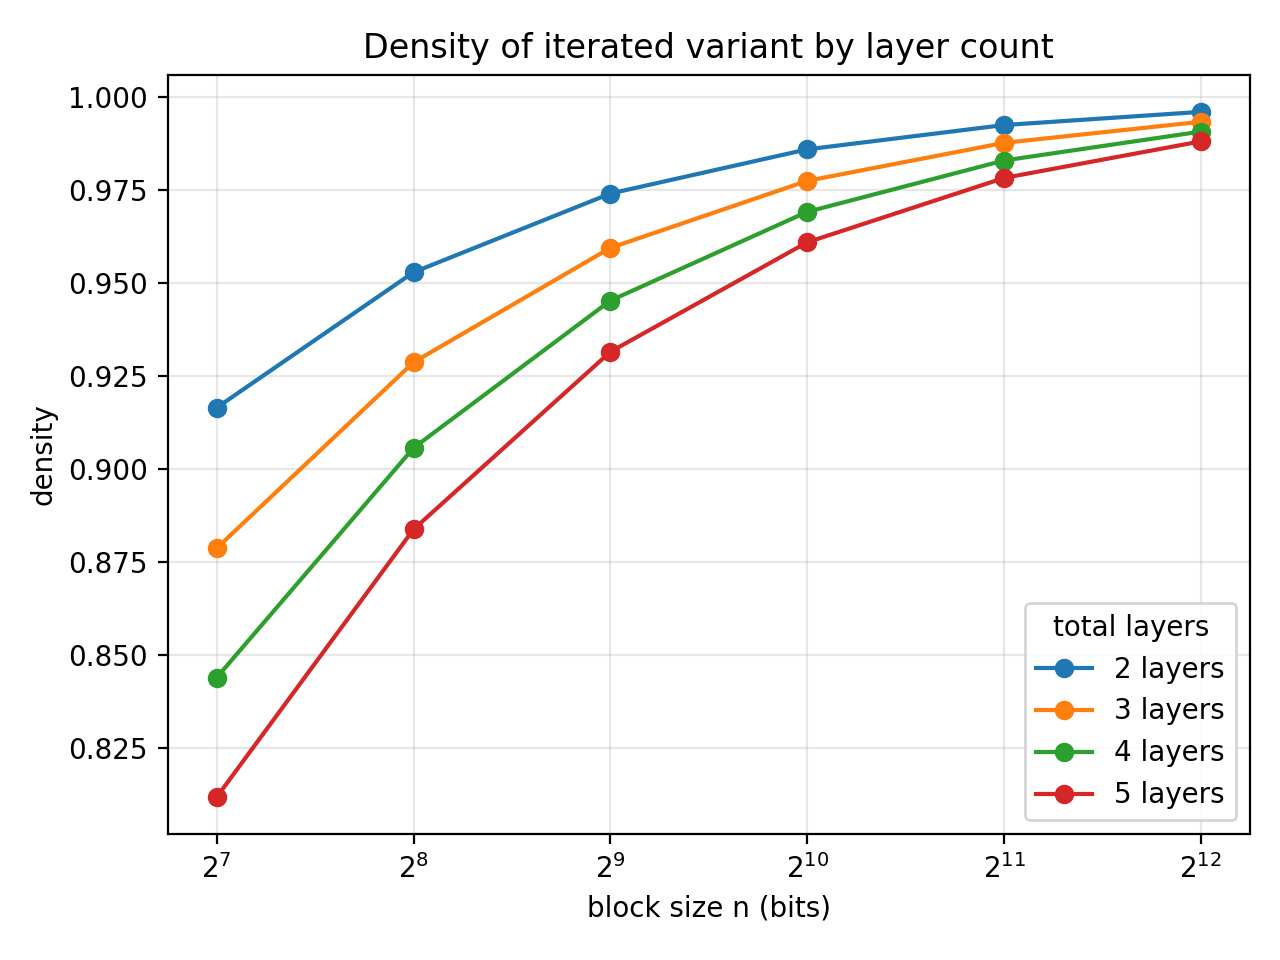
\includegraphics[width=0.9\textwidth]{../code/experiments/plots/iterated_layers_density.png}
    \caption{Public knapsack density of the iterated variant for different layer counts.}
    \label{fig:iterated-layers-density}
\end{figure}

\section{Influence of Key-Generation Parameters}

The implementation generates the private superincreasing sequence by adding a
small random increment to the current sum of previous weights. This increment
is controlled by the constant \texttt{MH\_DEFAULT\_DELTA\_MAX}. Larger values
can make the private weights grow faster. Because the reported density is based
on the bit length of the largest public weight, larger generated weights can
reduce the reported density.

Figure~\ref{fig:sweep-delta-density} shows this effect. For small block sizes,
larger increment values reduce the density more visibly. For example, for
\(n=128\), increasing \texttt{MH\_DEFAULT\_DELTA\_MAX} from \(1\) to \(128\)
changed the average density from \(1.000\) to about \(0.948\). For \(n=4096\),
the same change only reduced the average density to about \(0.998\). This
happens because the additional increment contributes only a small number of
extra bits compared with the full size of a long superincreasing sequence.

\begin{figure}[htbp]
    \centering
    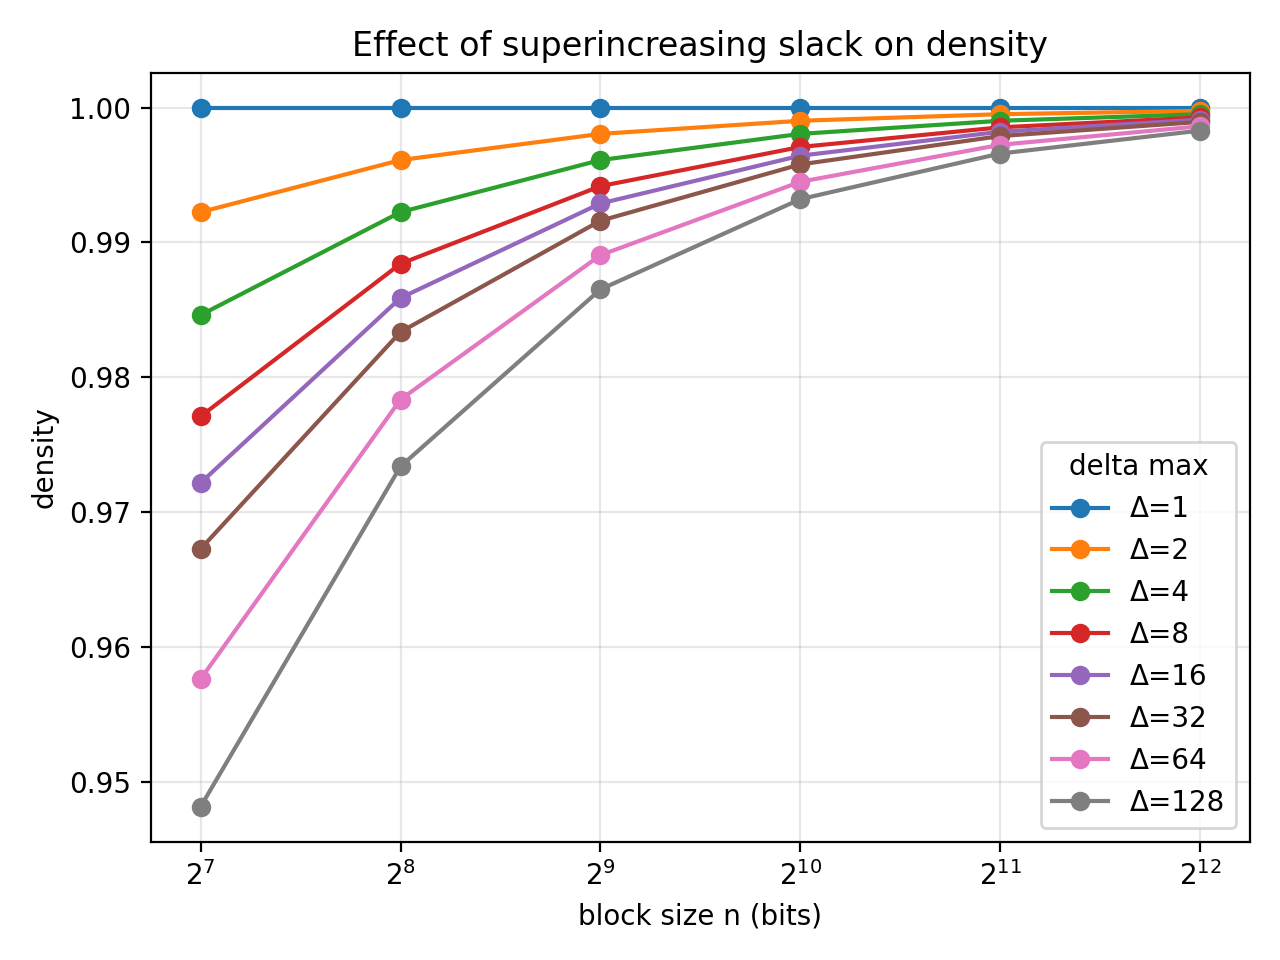
\includegraphics[width=0.9\textwidth]{../code/experiments/plots/sweep_delta_density.png}
    \caption{Effect of the superincreasing increment parameter on public knapsack density.}
    \label{fig:sweep-delta-density}
\end{figure}

The recorded bit length of the private-weight sum explains this trend.
Increasing \texttt{MH\_DEFAULT\_DELTA\_MAX} gives the generator more possible
choices for each private weight, but it also makes the generated values larger.
This creates a simple trade-off in this implementation between variation in the
private sequence and the size of the resulting key material. In the experiment,
increasing the increment bound from \(1\) to \(128\) raised the average
private-sum bit length from \(128\) to \(135\) bits for \(n=128\), and from
\(4096\) to \(4103\) bits for \(n=4096\). 

The sweep of the modulus margin had almost no visible effect on the reported
density. Increasing the margin bound changed how much larger the modulus was
than the sum of the private weights, but the bit length of the generated public
weights stayed almost unchanged. This is expected for this generator, because
the added margin is small compared with the private sum.

These results should be interpreted carefully. They only show how this
particular generator changes the measured density for the tested parameters and
do not prove resistance to lattice attacks. The density values are useful for
connecting the implementation with the theoretical discussion, but they are not
a complete security measure.

\section{Subset-Sum Solver Experiments}

The solver experiments compare brute-force search with meet-in-the-middle
search. They treat the public knapsack and ciphertext as a subset-sum instance
and try to recover the message vector. Brute force checks possible bit vectors
one by one, so its worst-case running time grows as \(2^n\). Meet-in-the-middle
splits the weights into two halves and compares partial sums. This reduces the
time growth, but it requires an exponential table of partial sums.

Figure~\ref{fig:attack-ms} shows the measured running time of both solvers. The
vertical axis is logarithmic. The brute-force solver becomes expensive already
for small values of \(n\). In these measurements, it was tested only up to
\(n=22\), where the average running time was about \(188\) ms. The
meet-in-the-middle solver handled larger values in this experiment. It reached
\(n=40\), where the average running time was about \(757\) ms.

\begin{figure}[htbp]
    \centering
    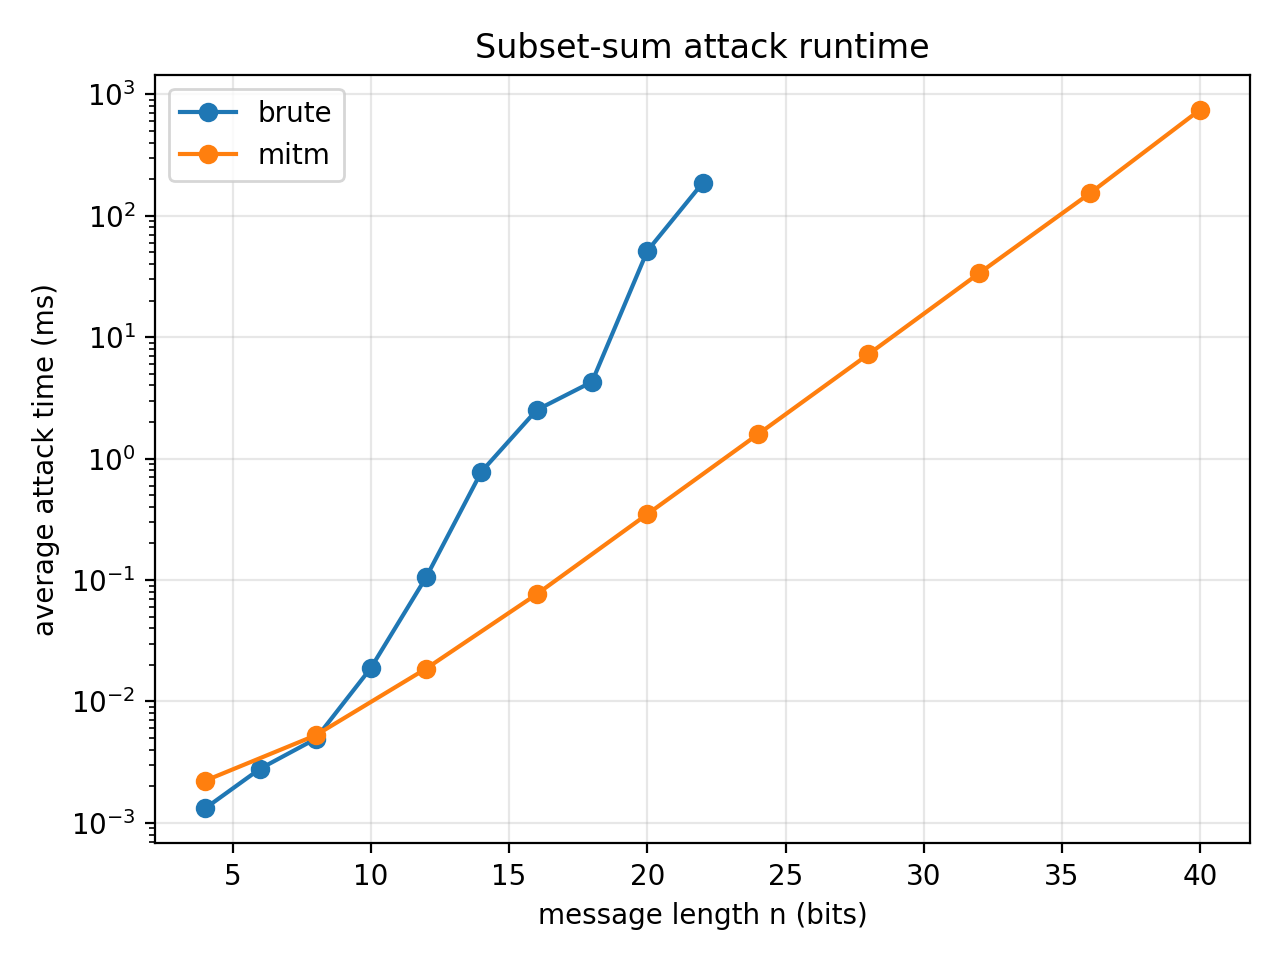
\includegraphics[width=0.9\textwidth]{../code/experiments/plots/attack_ms.png}
    \caption{Runtime of the implemented brute-force and meet-in-the-middle subset-sum solvers.}
    \label{fig:attack-ms}
\end{figure}

The meet-in-the-middle method is faster because it does not enumerate all
\(2^n\) full bit vectors directly. Instead, it stores partial sums for both
halves of the instance and searches for matching values. The trade-off is
memory usage. For an input of length \(n\), the implementation stores
\[
    2^{\lfloor n/2 \rfloor} + 2^{\lceil n/2 \rceil}
\]
table entries. Thus the table has \(131072\) entries for \(n=32\) and
\(2097152\) entries for \(n=40\). This is why the method is useful for larger
toy examples than brute force, but it still grows exponentially.

\section{Summary of Experimental Results}

The experiments confirm that the implemented schemes correctly perform key
generation, encryption, and decryption for the tested inputs. The runtime
measurements show that the implementation is fast for educational parameter
sizes, with key generation being the largest part of the cost in the classical
variant. The additional iteration experiment shows that more modular layers
increase the runtime and can lower the measured density of the public knapsack.
The parameter sweeps show that the construction of the private superincreasing
sequence influences density through the size of the generated weights, while the
modulus margin has little effect under this compact generator.

The subset-sum solver experiments show the increasing cost of direct
message-recovery methods. Meet-in-the-middle improves on brute force for the
tested sizes, but it still has exponential time and memory requirements. These
results are useful as an experimental baseline. They should not be confused
with the main cryptanalytic attacks on Merkle--Hellman, which exploit the
structure of the generated public key rather than only enumerating possible
messages.
